
\documentclass[a4paper, 10pt]{IEEEconf}  

\usepackage{geometry}
\geometry{a4paper, margin=1in}
    
\usepackage{verbatim}
\usepackage{graphicx}
\usepackage{pdfpages}
\usepackage{cite}
\usepackage{listings}
\usepackage{float}
\usepackage{url}
\usepackage{hyperref}
\usepackage{fancyhdr}

\lstset{
	tabsize=2,
	breaklines=true
}

\setlength{\parskip}{1em}
\onecolumn

\title{\LARGE \bf Project 1: Pneumatic Cylinder\\Mechatronics  282 778}
\author{Marc Alexander Sferrazza \\ 12164165
\thanks{This work was not supported by any organization}
\thanks{Faculty of Mechatronics Engineering, Massey University, Albany, Auckland, New Zealand
        {\tt\small Progress of project: https://github.com/alex1v1a/Mechatrnoics/} } }

\begin{document}

\maketitle

%\begin{figure}[H]
%  \includegraphics[width=\linewidth]{images/final}
%  \label{fig:Final Product}
%\end{figure}

\thispagestyle{empty}
\pagestyle{plain}


%%%%%%%%%%%%%%%%%%%%%%%%%%%%%%%%%%%%%%%%%%%%%%%%%%%%%%%%%%%%%%%%%%%%%%%%%%%%%%%%

\begin{abstract}

Pneumatic actuation controlled project involving the projection of tennis balls. The projectiles are deployed from the actuation controlled device at fixed intervals and have an optional override to deploy manually. 
\\

The project involves constructing a frame in which will enclose and secure all parts in an orderly safe fashion; designing and building the PCB circuit with the consideration of controlling the solenoid, reading and displaying the extension of the actuator.
\\

In this process, acquired Mechatronics skills are tested to build a devices which has mechanical, electrical and programming components with consideration of materials properties. To utilise all of the skills on a basic level of which can measure the performance and aptitude of converging these skills, and how things are done individually. While there are many methods to preform the task, consisting of different professional approaches is key for performance on an industry level.

\end{abstract}


\clearpage
\tableofcontents
\listoffigures
%\listoftables
\thispagestyle{empty}
\clearpage
\twocolumn

%%%%%%%%%%%%%%%%%%%%%%%%%%%%%%%%%%%%%%%%%%%%%%%%%%%%%%%%%%%%%%%%%%%%%%%%%%%%%%%%
%%%%%%%%%%%%%%%%%%%%%%%%%%%%%%%%%%%%%%%%%%%%%%%%%%%%%%%%%%%%%%%%%%%%%%%%%%%%%%%%

\setcounter{page}{1}

\section{INTRODUCTION}

The project is to utilise skills acquired, to build a mechatronic device that uses an actuation and sensing sub-system, with a control interface to time the interval in which it takes to deploy a projectile (tennis ball) from the hopper. The interface will display the extension of the actuator on an LCD display. The hopper can hold up to 3 projectiles (tennis balls) which are pre-loaded, and will deploy with a fixed time interval or manual override ejection.

%%%%%%%%%%%%%%%%%%%%%%%%%%%%%%%%%%%%%%%%%%%%%%%%%%%%%%%%%%%%%%%%%%%%%%%%%%%%%%%%

\subsection{Aims \& Objectives}

To build a mechatronic sub-system device, integrating actuation, sensing, and control sub-systems.

The key objectives to cover in this task includes

\begin{itemize}
	\item Control the extension and contraction of a pneumatic cylinder.
	\item Measure the extension and contraction of a pneumatic cylinder.
	\item Integrate the mechatronic actuation, sensor, and control sub-systems in order to eject projectiles from a hopper with a fixed time period between deployments.
\end{itemize}

There are no constraints at which the design is to be achieved, leaving the best found method determined by the development. Therefore the process and development in the design is open for opinion given appropriate reasoning.

%%%%%%%%%%%%%%%%%%%%%%%%%%%%%%%%%%%%%%%%%%%%%%%%%%%%%%%%%%%%%%%%%%%%%%%%%%%%%%%%
%%%%%%%%%%%%%%%%%%%%%%%%%%%%%%%%%%%%%%%%%%%%%%%%%%%%%%%%%%%%%%%%%%%%%%%%%%%%%%%%

\section{METHOD}

A detailed description of what was done, how, and why. 

%%%%%%%%%%%%%%%%%%%%%%%%%%%%%%%%%%%%%%%%%%%%%%%%%%%%%%%%%%%%%%%%%%%%%%%%%%%%%%%%

\subsection{Frame Material Selection}

Planning in design for structural integrity is subject to the workspaces constraints, while there are many methods of which the design can be achieved, in a long life usage of the project using metals can prove effective; however in the projects scope the projectiles may be launched a minimum of eight times effectively without damage to the chassis. Therefore the design materials are chosen subject to a prototype friendly, cost effective method which will meet the required eight successful launches for demonstration and any additional deployment during testing and compensation of the demonstration. 

The estimated reasonable number of ejections required used is 100 cycles of both extension and contraction for the pneumatic cylinder, as this is the highest action point of the device, while all other parts remain fixed except the projectiles themselves. 

With considerations of this, and analysis provided such as FEA strain tests over 200 (double the required) cycles with Solidworks 2015 and the isolated actuation frame the selected material chosen is entirely based on acrylic with the exception of PVC piping (explained further in frame design for the hopper pre-load). 

\begin{figure}[H]
  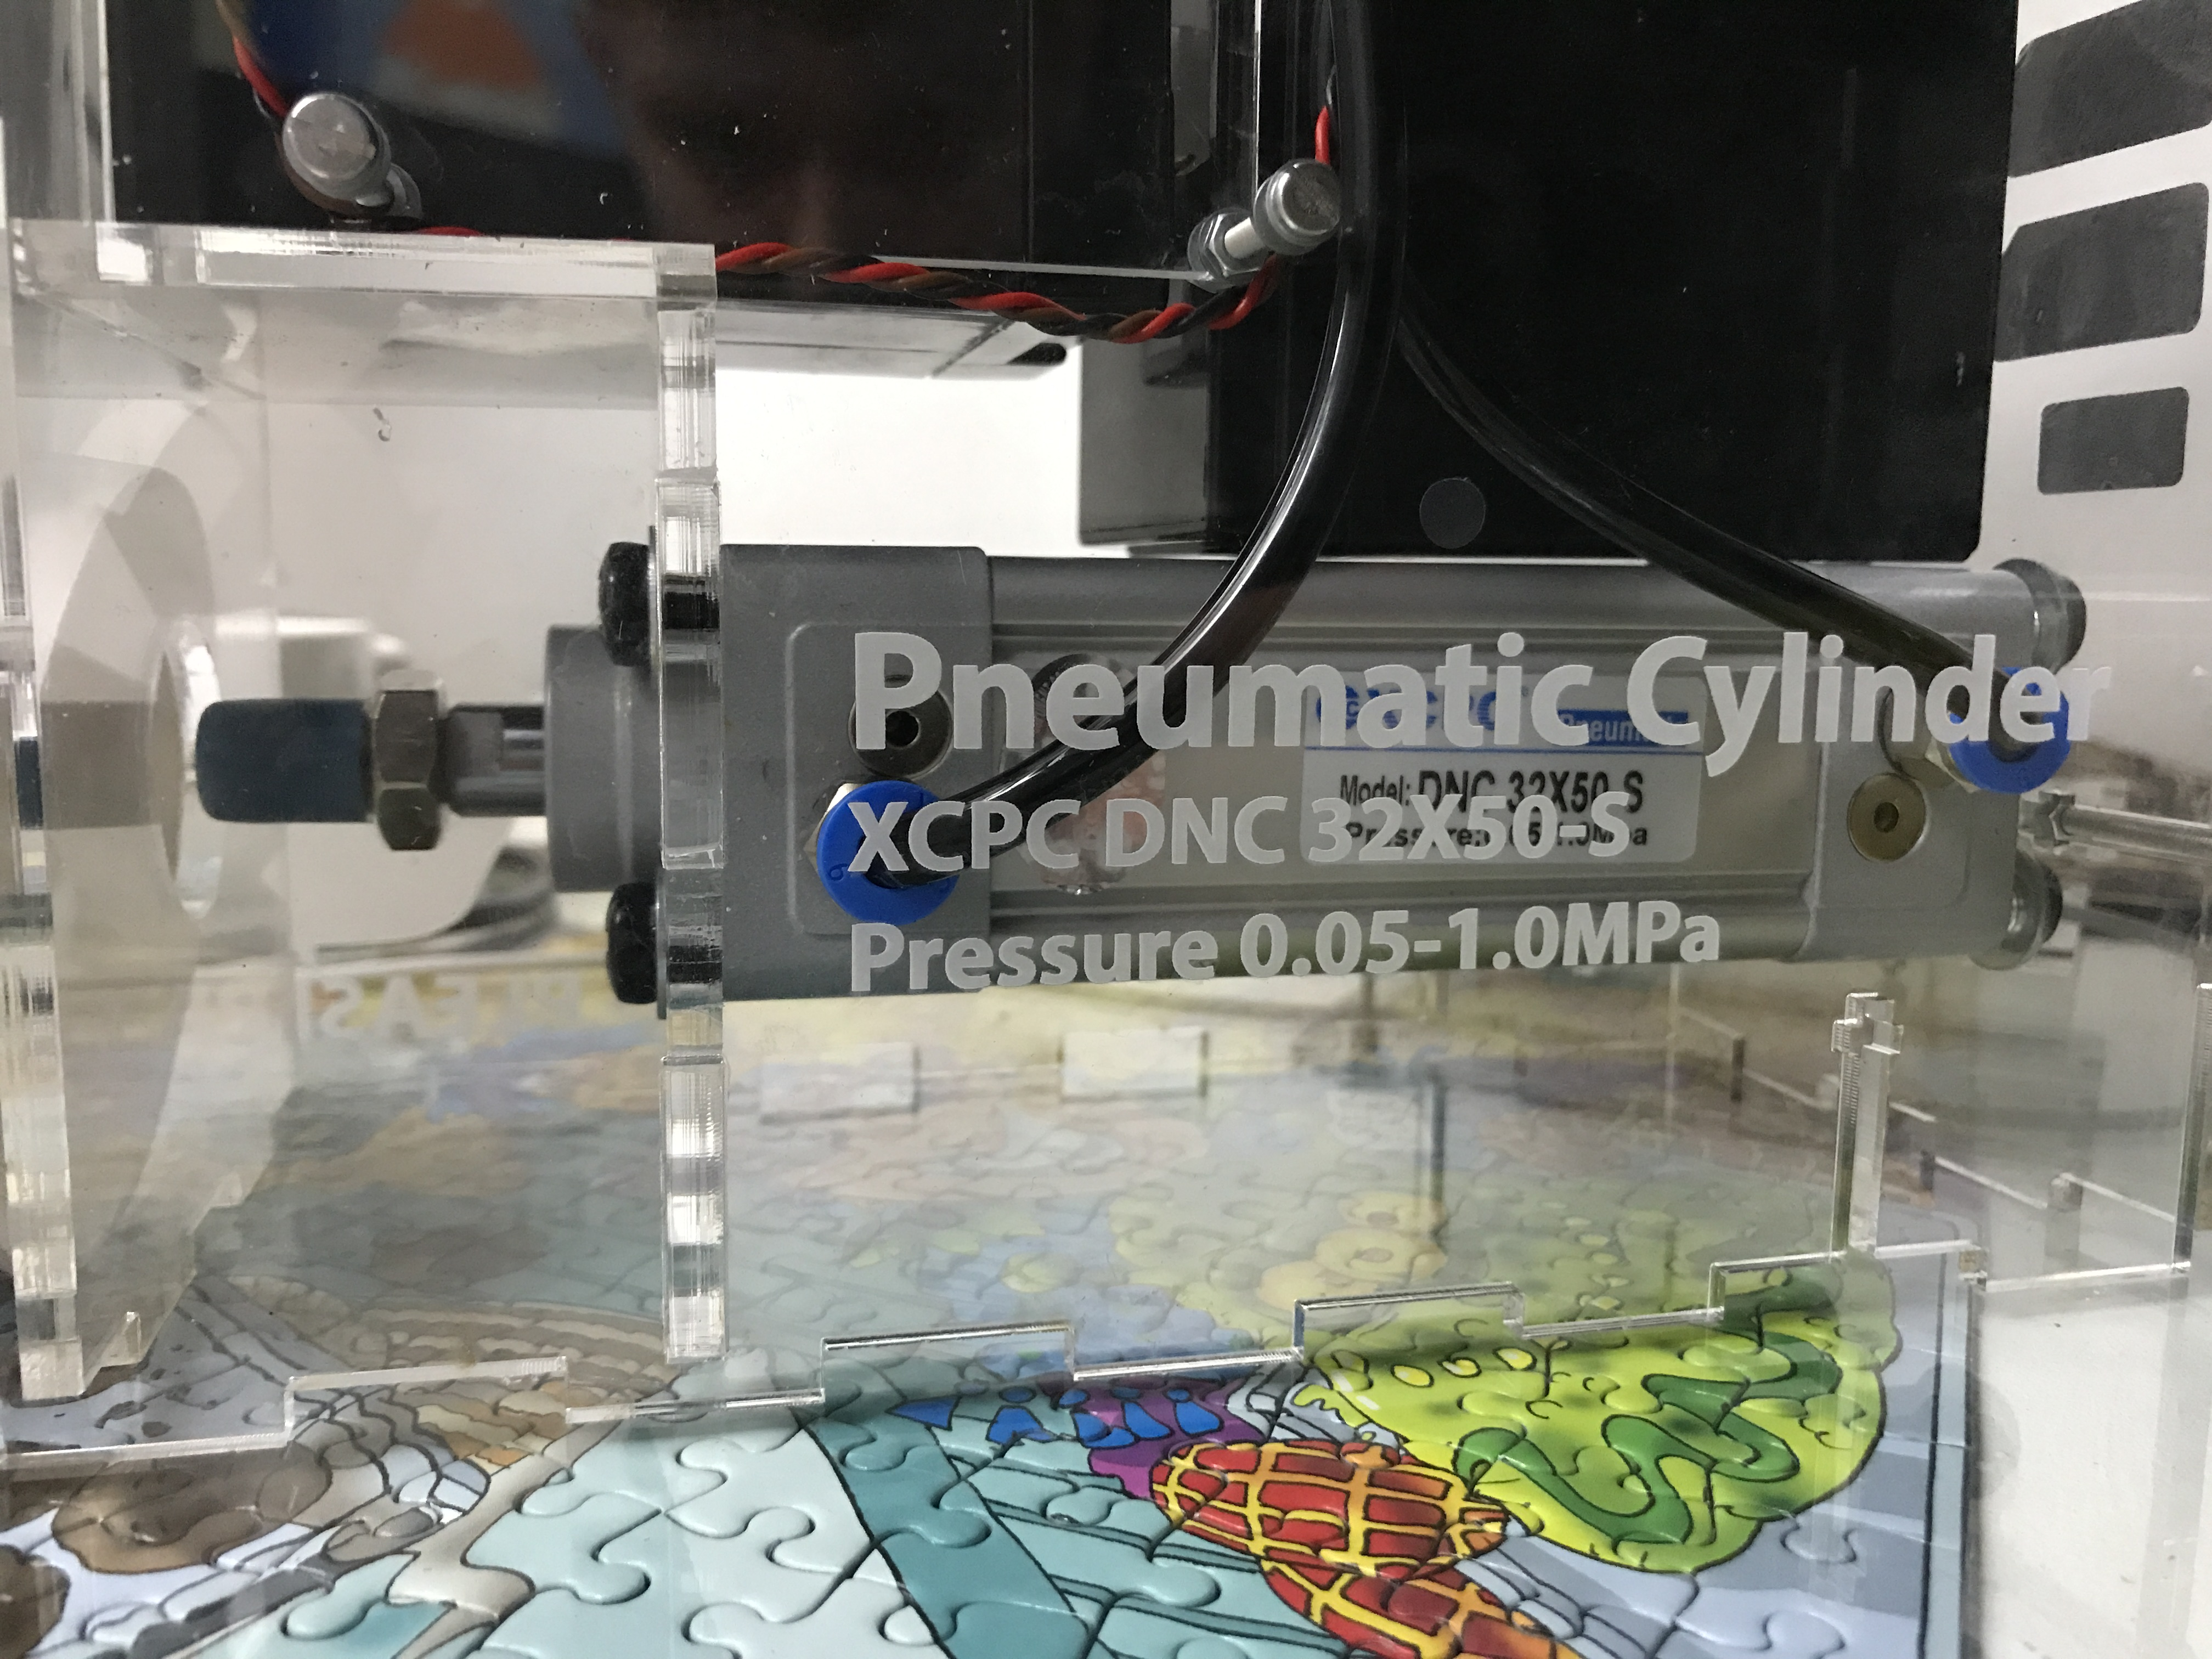
\includegraphics[width=\linewidth]{images/cylinder}
  \caption{Isolated actuation frame}
  \label{fig:Isolated actuation frame}
\end{figure}

While acrylic is more brittle then other ready available materials such as MDF, acrylic has the beneficial key feature of being fully transparent, so a full display of all parts can be monitored, and the full demonstration of all internal parts can be observed. Another key reason for this choice in material is the bonding of surfaces in the respect that with specific chemicals applied the surfaces fuse together and become bonded, almost in the sense they were moulded that way which with correct design can spread force through the entire chassis.


%%%%%%%%%%%%%%%%%%%%%%%%%%%%%%%%%%%%%%%%%%%%%%%%%%%%%%%%%%%%%%%%%%%%%%%%%%%%%%%%

\subsection{Frame design}

For the frames design it is important to have a clean and functional, practical layout, so that all components have an appropriate amount of space and remain somewhat easily accessible. The enclosure should be safe with no hazardous features such as electric safety and sharpe edges to be cut on. As this is not a final manufacturable product, and rather more towards a prototype model the features are not strict on including mould casting and perfect rounded edges, but still somewhat of a safe standard with no edge lifting and fused surfaces to maintain integrity. 

The frames design will be used as not only the containing housing, but also as a key point in the systems integrity. This is due to the force load's shock being dissipated over a compression surface rather then stressed all on a single point. The design features this to allow the acrylic to slightly expand on each deployment of a projectile, and in the expansion stage to lengthen the duration of the force to ensure the enclosure will not crack for the expected life cycles. This is the fundamental key aspect when designing the enclosure, along side the secure fitment and spacing of all components. 

The material selection of acrylic and PCV piping is a cheap and effective way for rapid prototyping, and has not only has great functionality in this design, but also allows assessment of the internal design with the transparent enclosure. The selected PVC pipe (80mm) for hopper to contain the pre-loaded projectiles, and a more accurate deployment has been chosen as it is a cheap and effective method of storing, with a compensation of 6-10mm each side (An internationally recognised tennis balls diameter is 65.4–68.6mm) \cite{ball} of the projectile. While it has been difficult to cut the piping accurately a 'T' pipe has be used rather then assembling a custom joint as this was found to be a better method.

Below is a figure of the rapid prototyping process. The parts are laser cut, and another beneficial aspect of this is that if any part shall unfortunately break for whatever reason, a replacement part can be cut with little effort.

\begin{figure}[H]
  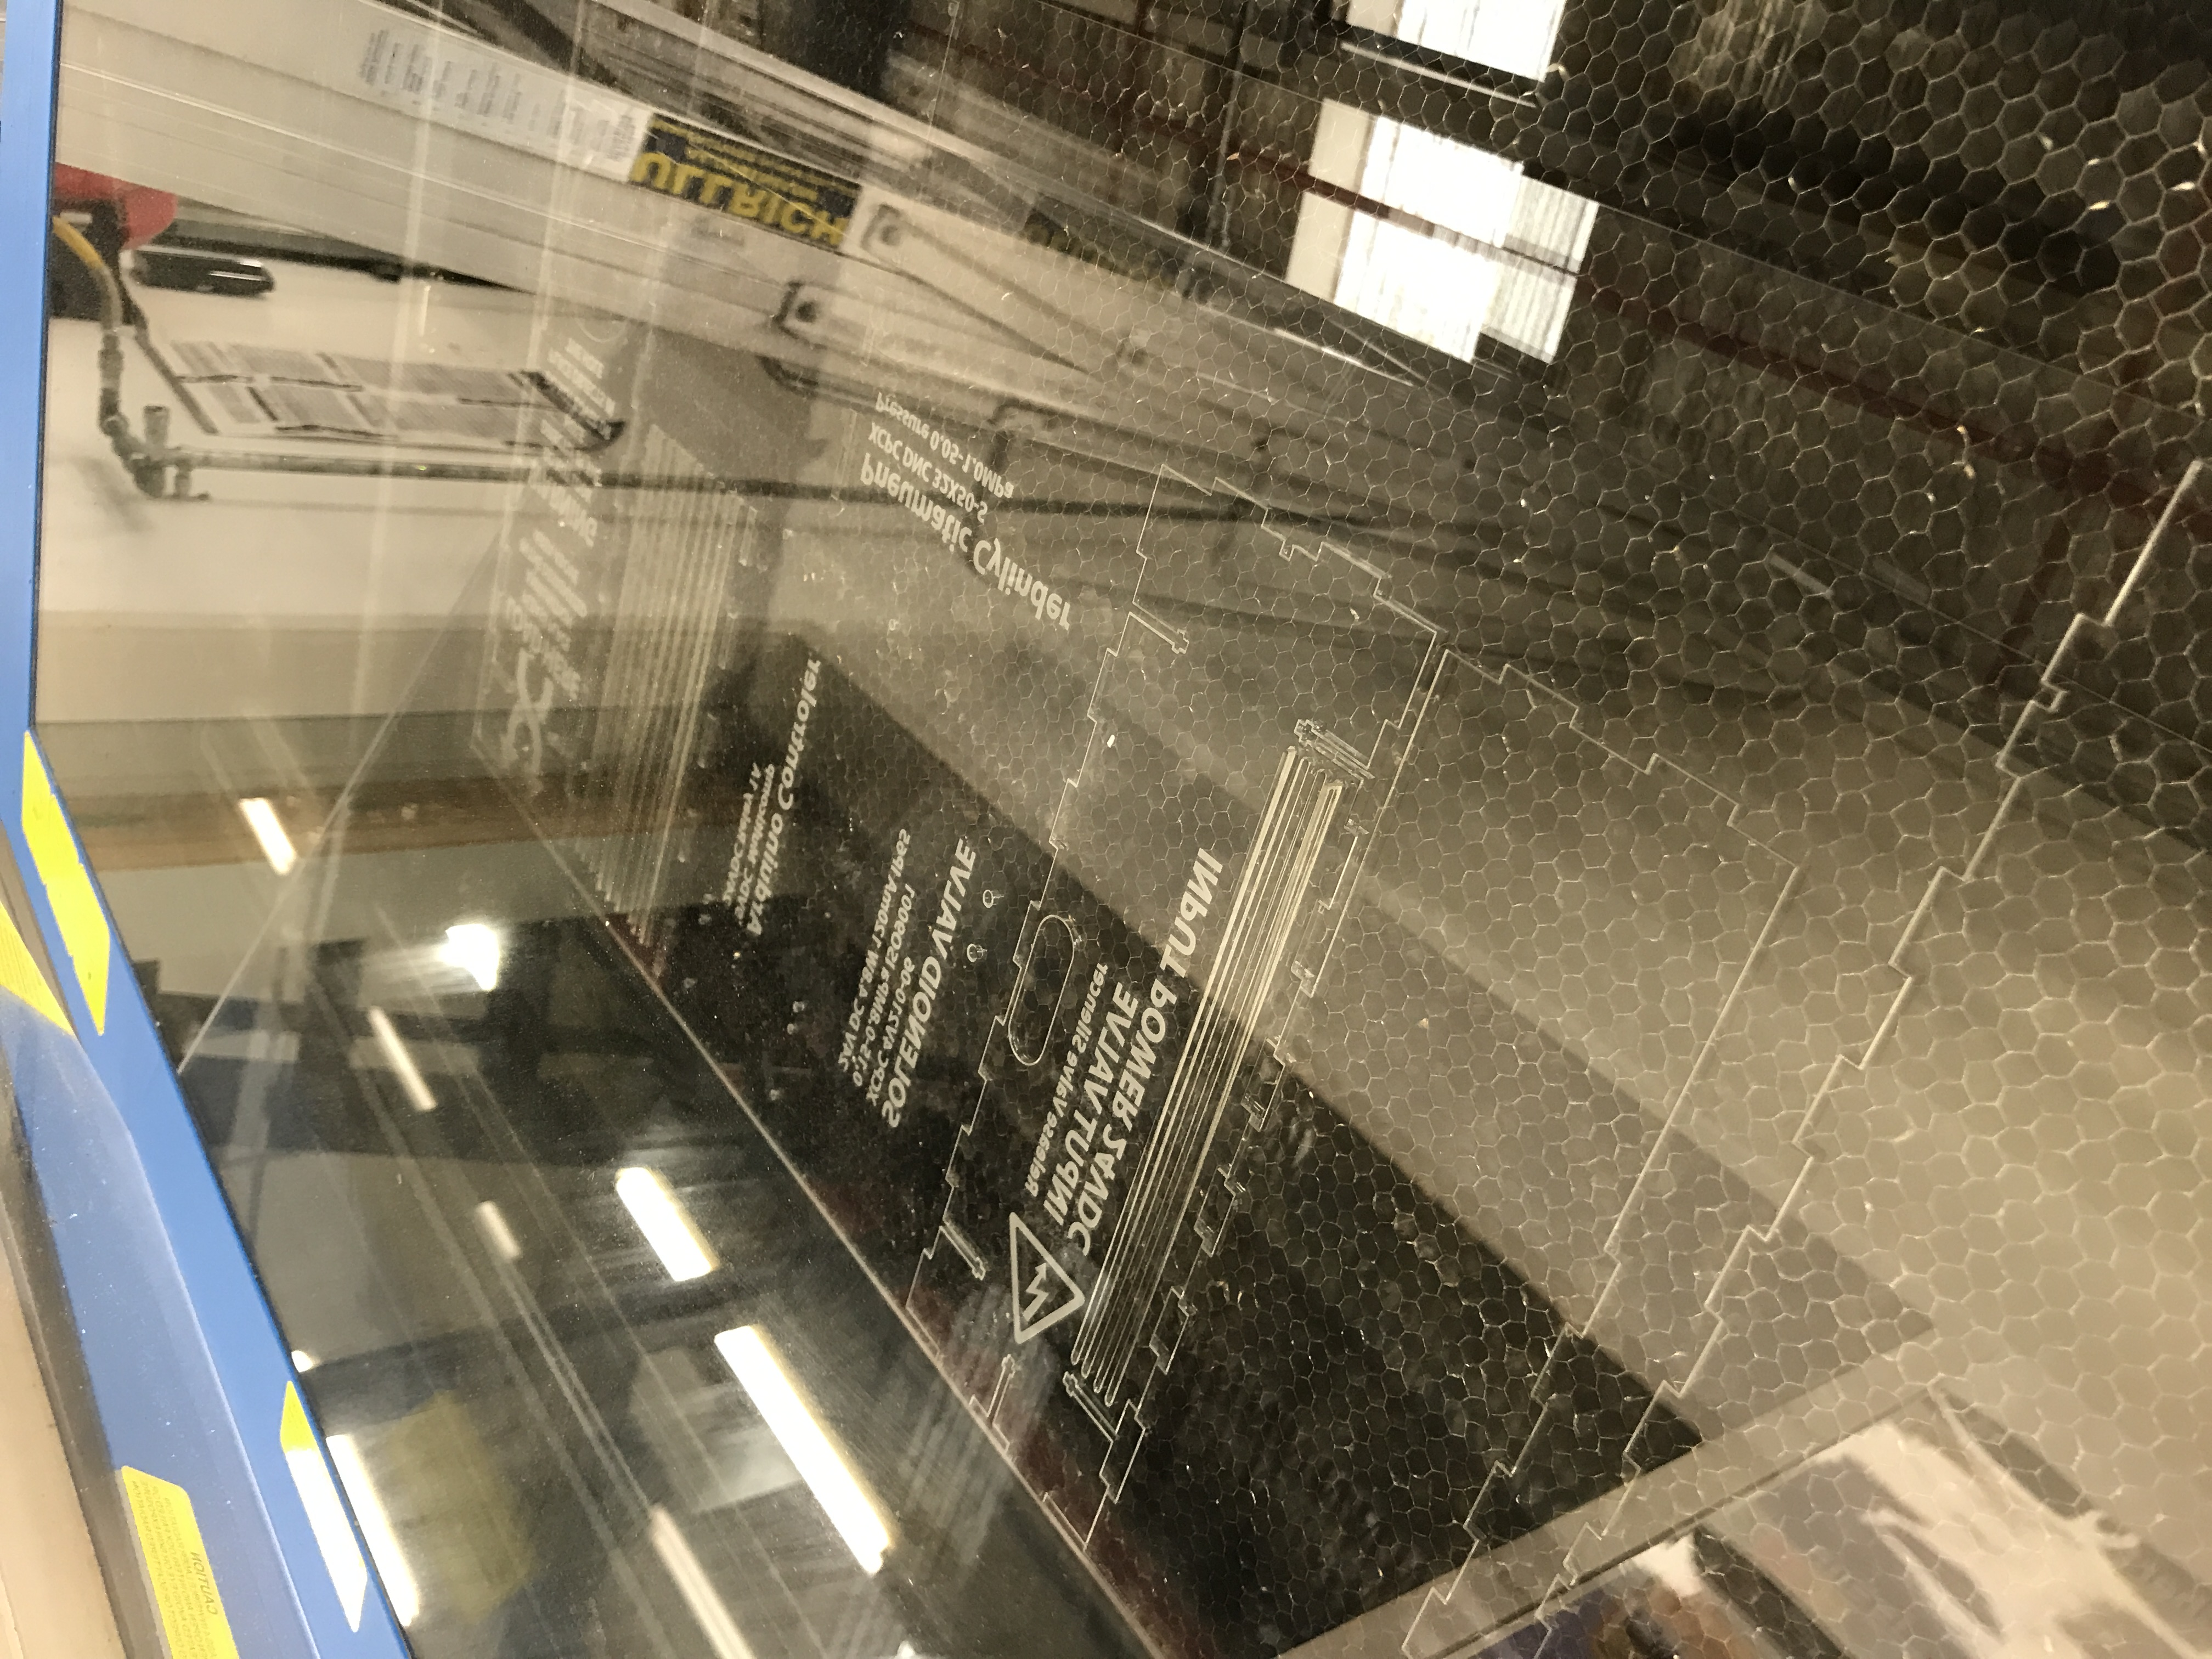
\includegraphics[width=\linewidth]{images/laser}
  \caption{Laser cutting the frame}
  \label{fig:Laser cutting the frame}
\end{figure}

Shown below is the base frame assembly with the solenoid and pneumatic actuator.

\begin{figure}[H]
  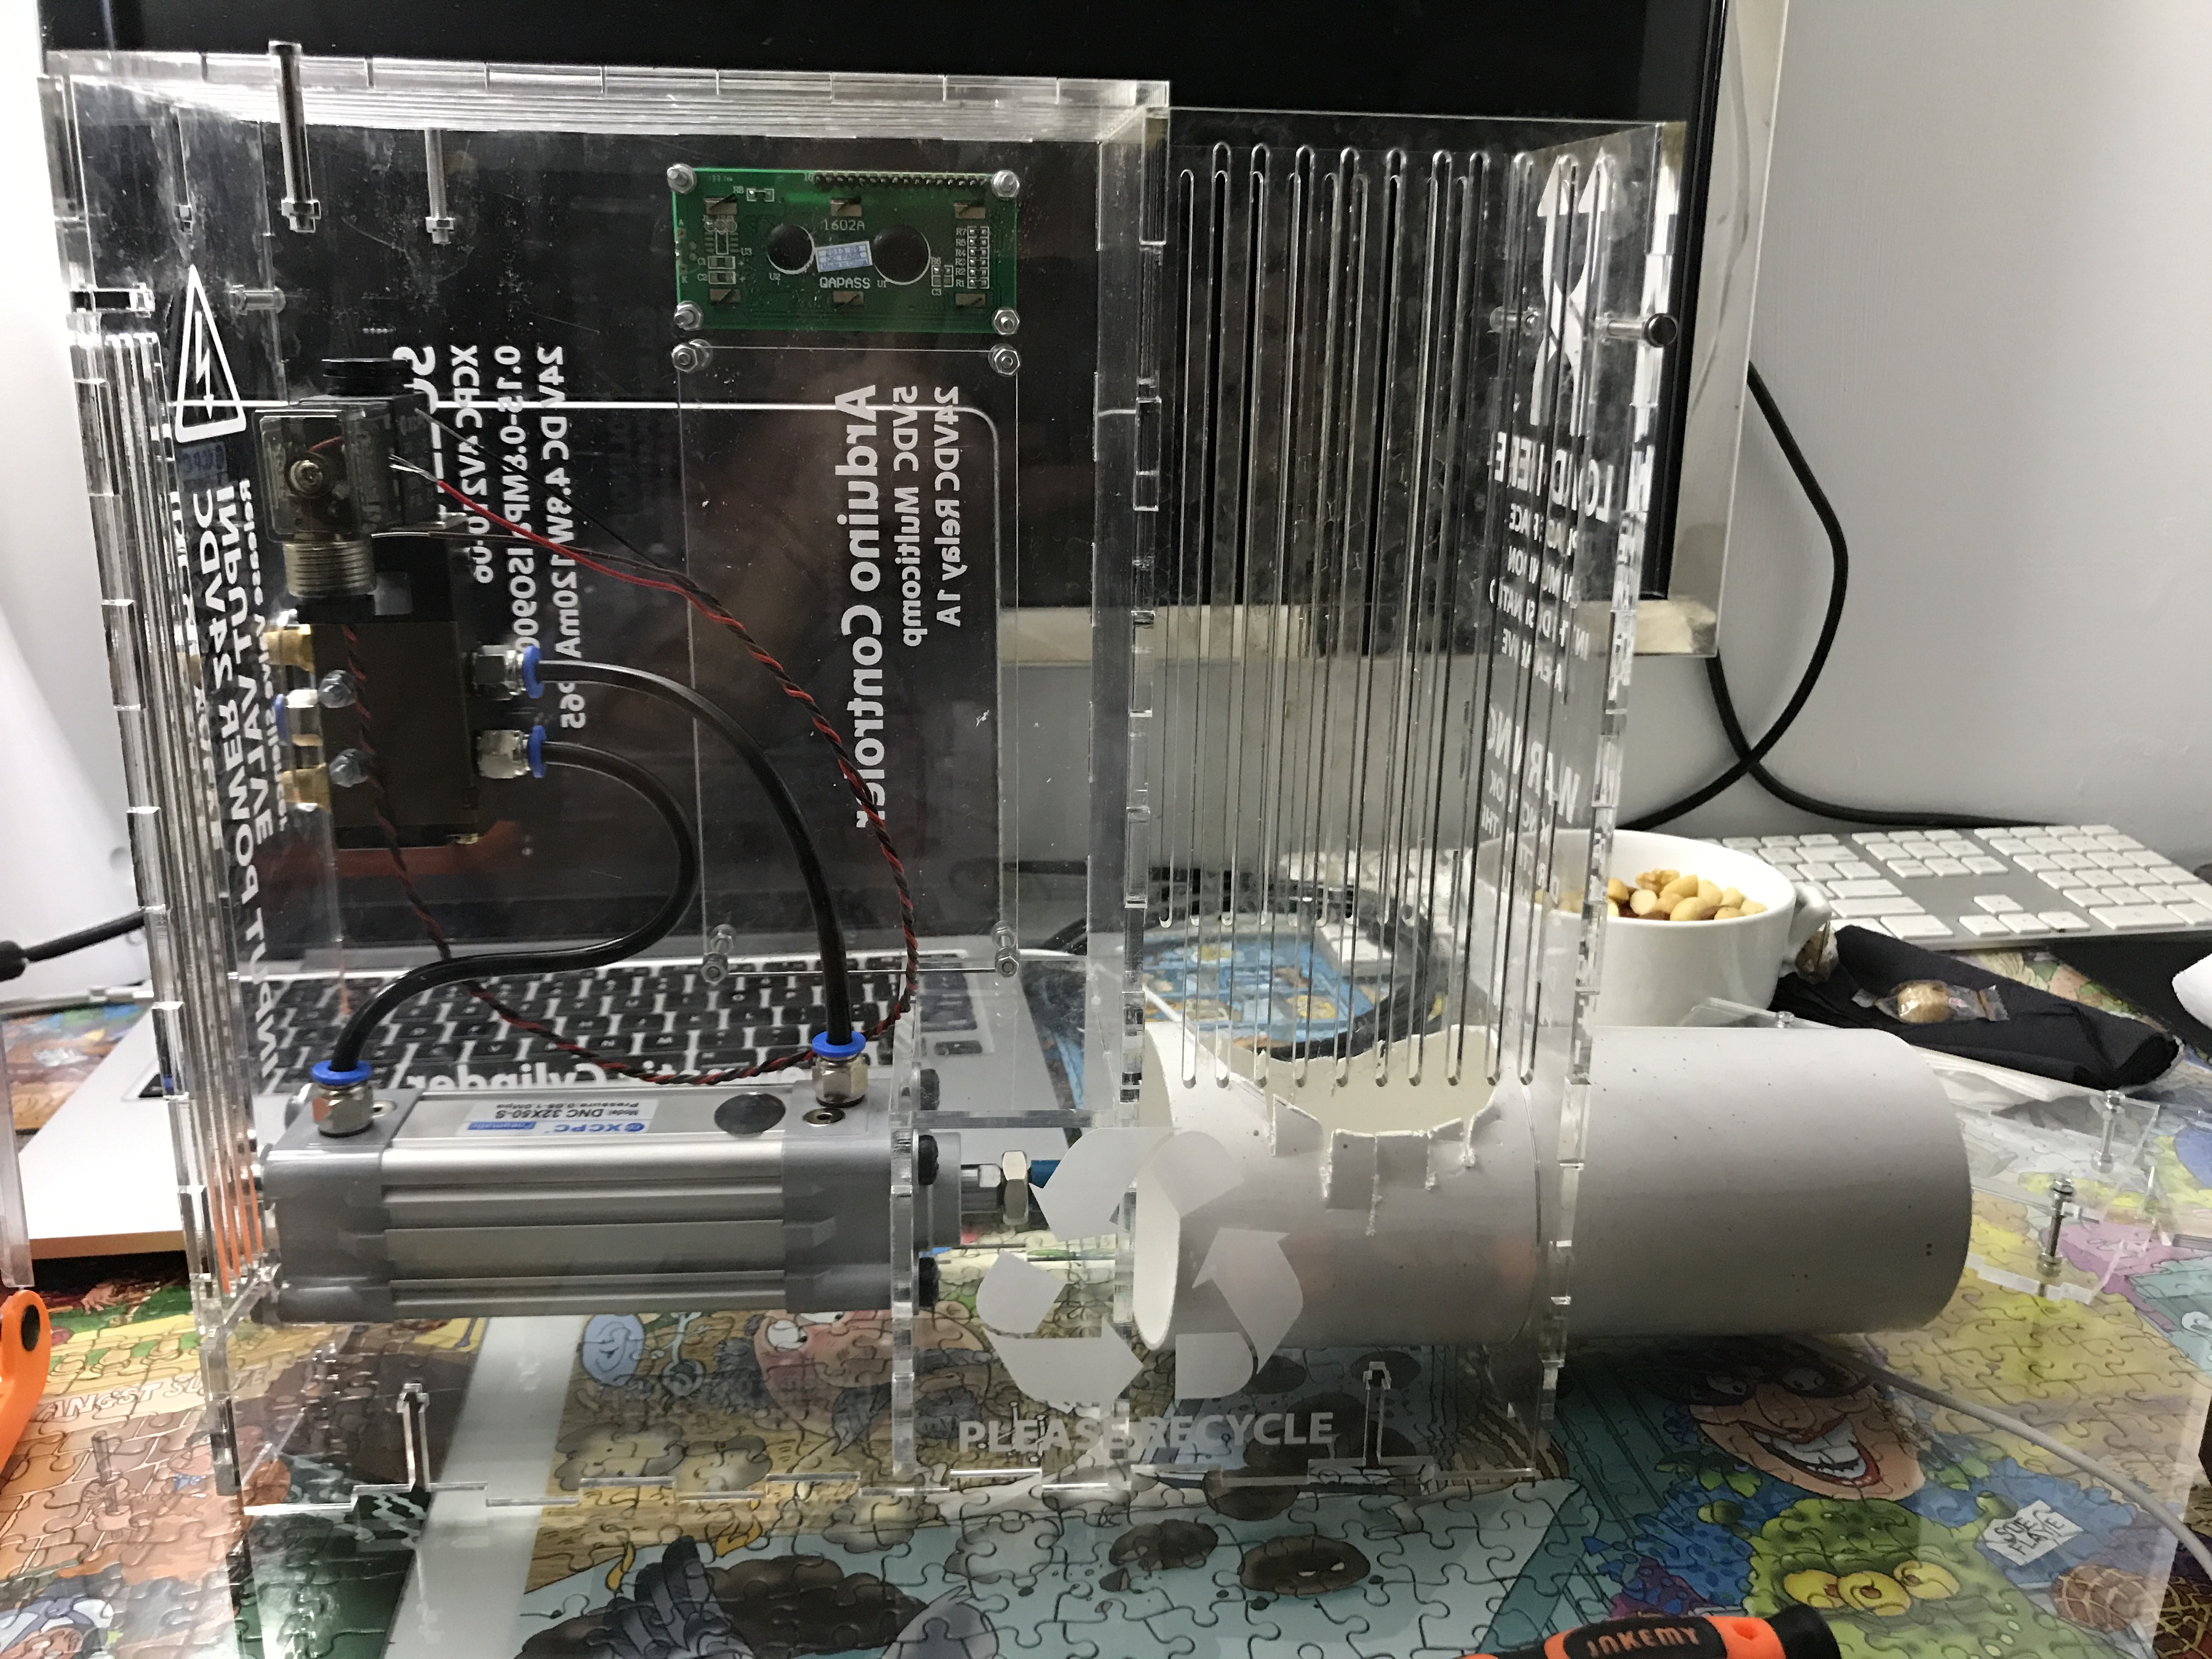
\includegraphics[width=\linewidth]{images/Frame}
  \caption{Basic stripped frame before population}
  \label{fig:Basic stripped frame before population}
\end{figure}

%%%%%%%%%%%%%%%%%%%%%%%%%%%%%%%%%%%%%%%%%%%%%%%%%%%%%%%%%%%%%%%%%%%%%%%%%%%%%%%%

\subsection{Bonding \& Linkages}

To secure the frame M3 30mm bolts and nuts were used with 8xM6 bolts securing the pneumatic actuator. All mounting and fastening of internal components is also achieved with M3 size bolts, while dampening foam has been used to cushion some surfaces.

The primary influence in structure bonding is C105 also known as acrylic weld but not to be mistaken with C502 also known as super glue for plastics and rubbers, which offers a different method of molecular bonding of surfaces. The advantage of C105 is that it is extremely thin comparable with water and preforms quick bonding which results in two or more surfaces being fused like overlaying corrugated iron.

The 105 Acribond contains
\begin{itemize}
	\item U.N. 1593 METHYLENE CHLORIDE CAS No. 75-09-2
	\item U.N. 1710 TRICHLOROETHYLENE STABILIZED CAS No. 79-01-6
	\item U.N. 1247 METHYL METHACRYLATE MONOMER CAS No. 80-62-6
\end{itemize}
PG III, HAZCHEM CODE 2Z, Class 6.1

For a more in depth discussion on bonding materials and useful chemistry for plastics and rubbers ePlastics website is linked in the reference section \cite{ePlastic}; the 105 Acribond link \cite{105} is also provided.

%%%%%%%%%%%%%%%%%%%%%%%%%%%%%%%%%%%%%%%%%%%%%%%%%%%%%%%%%%%%%%%%%%%%%%%%%%%%%%%%

\subsection{Power Supply}

The available option of a 24VDC bench power supply is provided, however for ease of use in testing and probability an internal power supply has been integrated. The selected cells are 2x 12VDC 7AH Gel AGM SLA batteries connected in series to provide a stable constant reliable power source which does not require frequent charging. The resultant supply is 24VDC 7AH for reference. 

There is a built in universal charge port using banana sockets of which any appropriate SLA 24V charger can be used. Due to the nature of the batteries and the self maintenance hydrogen gas released the frame includes vents for any build up of gas or excess heat from components.

\begin{figure}[H]
  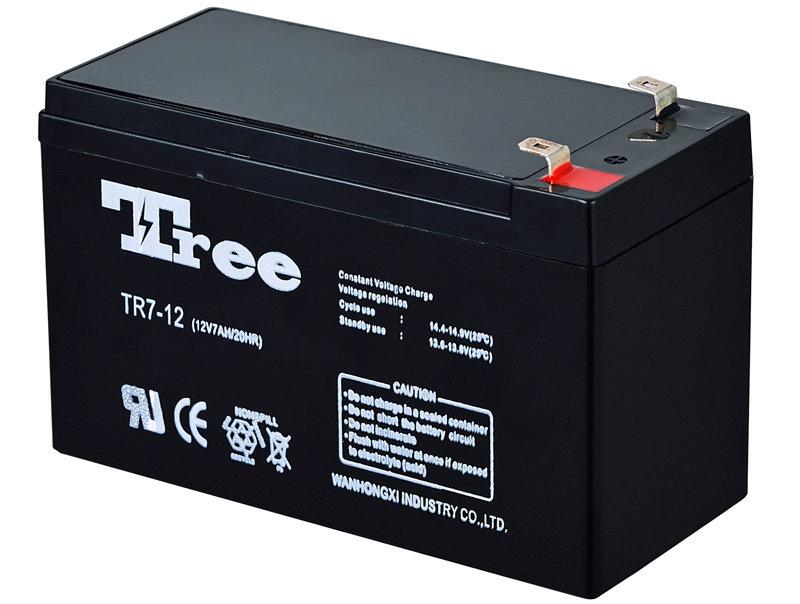
\includegraphics[width=\linewidth]{images/Battery}
  \caption{Tree Battery 12VDC 7AH Gel AGM SLA}
  \label{fig:Basic stripped frame before population}
\end{figure}

%%%%%%%%%%%%%%%%%%%%%%%%%%%%%%%%%%%%%%%%%%%%%%%%%%%%%%%%%%%%%%%%%%%%%%%%%%%%%%%%

\subsection{Eagle PCB}

Using Eagle CAD-soft from Autodesk \cite{eagle} a PCB is designed and implimented. 

The PCB design includes the following
\begin{itemize}
	\item Arduino controller
	\item Voltage regulator (24VDC to 5VDC)
	\item Relay from the Arduino to the solenoid (5VDC to 24VDC/120VDC 1A)
	\item Relevant LED's
	\item Safety features e.g. fuses (0.5A)
	\item Ground Core
\end{itemize}

The components are shown in a working order below. The LED's indicate the state of each action, with the red LED relating to power from the source at each stage 24VDC. Yellow being the state of the stage after some processing, the first being the regulation from 24VDC to 5VDC, the second being the normally closed side of the relay or contraction of the actuation arm. Finally the green LED is for the extension state of the actuation arm. These LED's are for status states only and debugging thus why they are not mounted and displayed on the enclosure although visible.

\begin{figure}[H]
  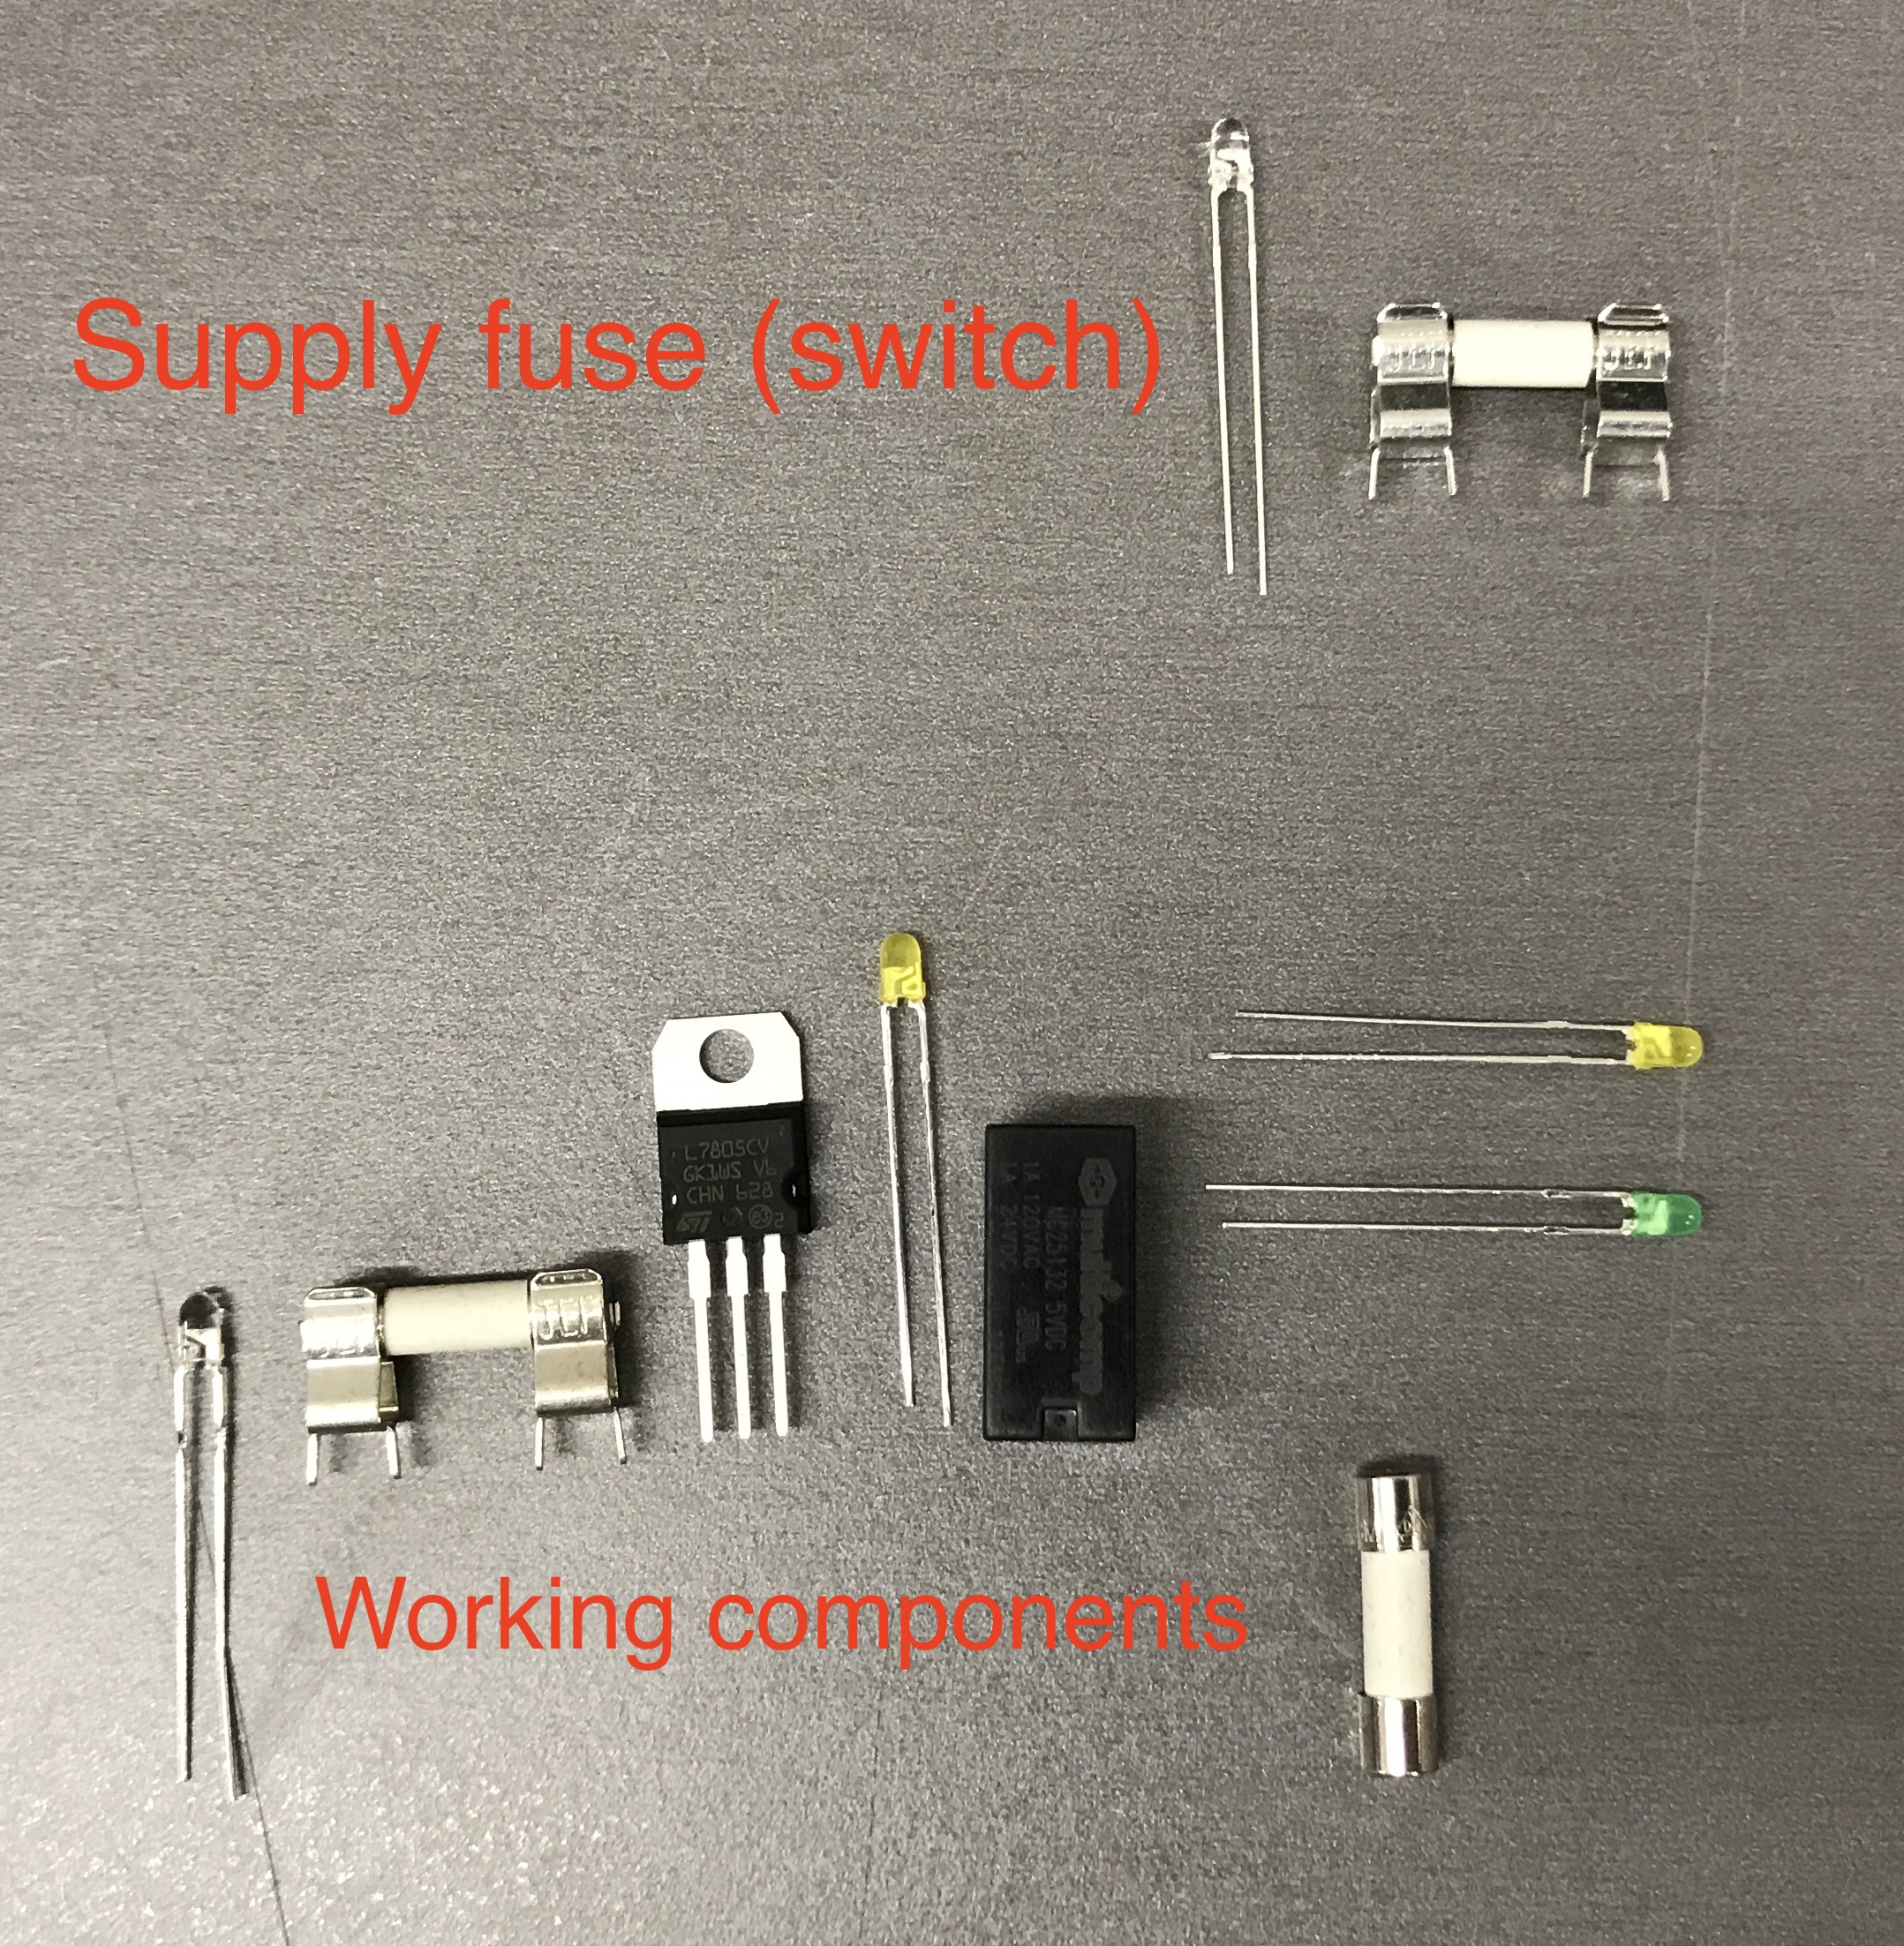
\includegraphics[width=\linewidth]{images/parts}
  \caption{Components of design}
  \label{fig:Components of design}
\end{figure}

A schematic of the design is given below. The design does not include capacitors after the regulator (or an attached heatsink) due to the current draw being less the 20\% of the capacity of the transistor which is 1A and is not required.

\begin{figure}[H]
  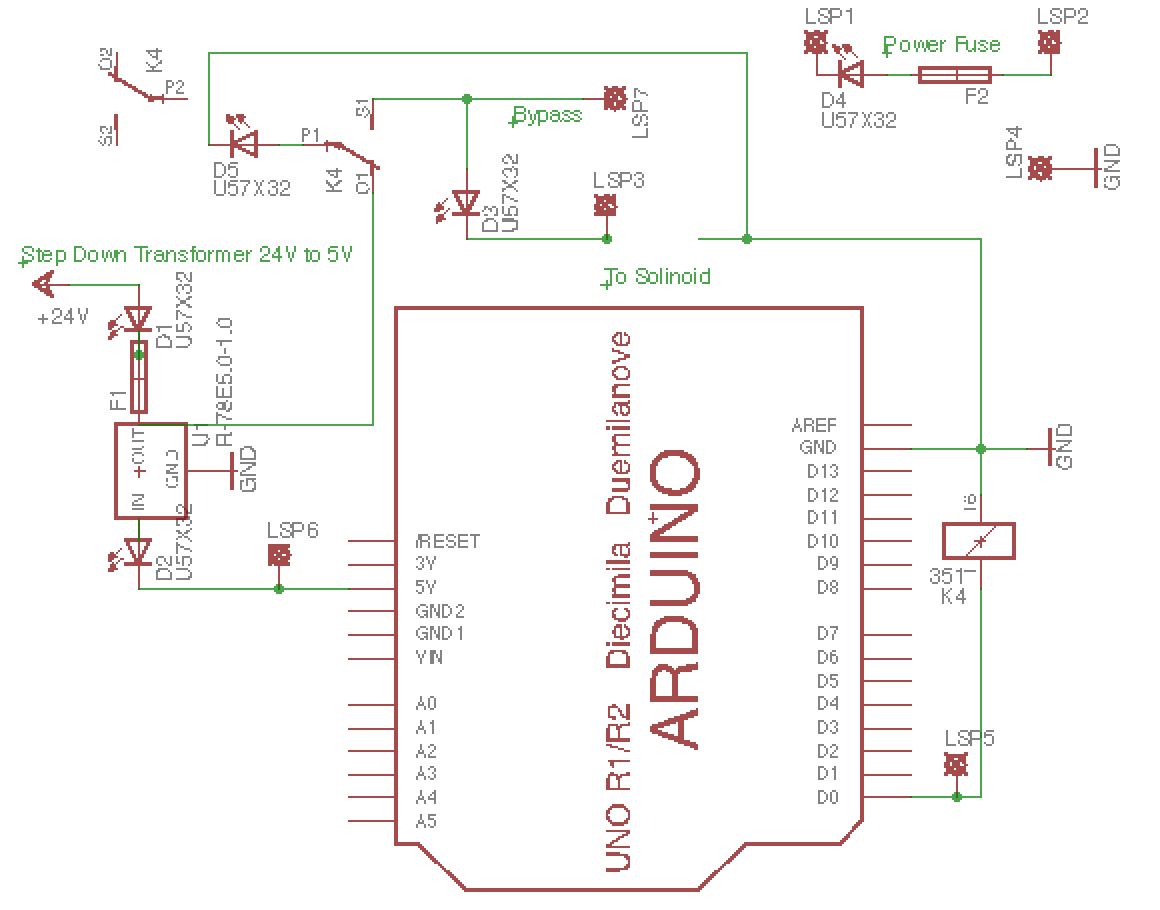
\includegraphics[width=\linewidth]{images/Schematic}
  \caption{Schematic}
  \label{fig:Schematic}
\end{figure}

The board drill out design is shown below. The purpose of this layout being a seperate entity rather then a shield of the Arduino, this is for display purposes only, and to preform visual inspection from the exterior of the enclosure for assessment and debugging. 

\begin{figure}[H]
  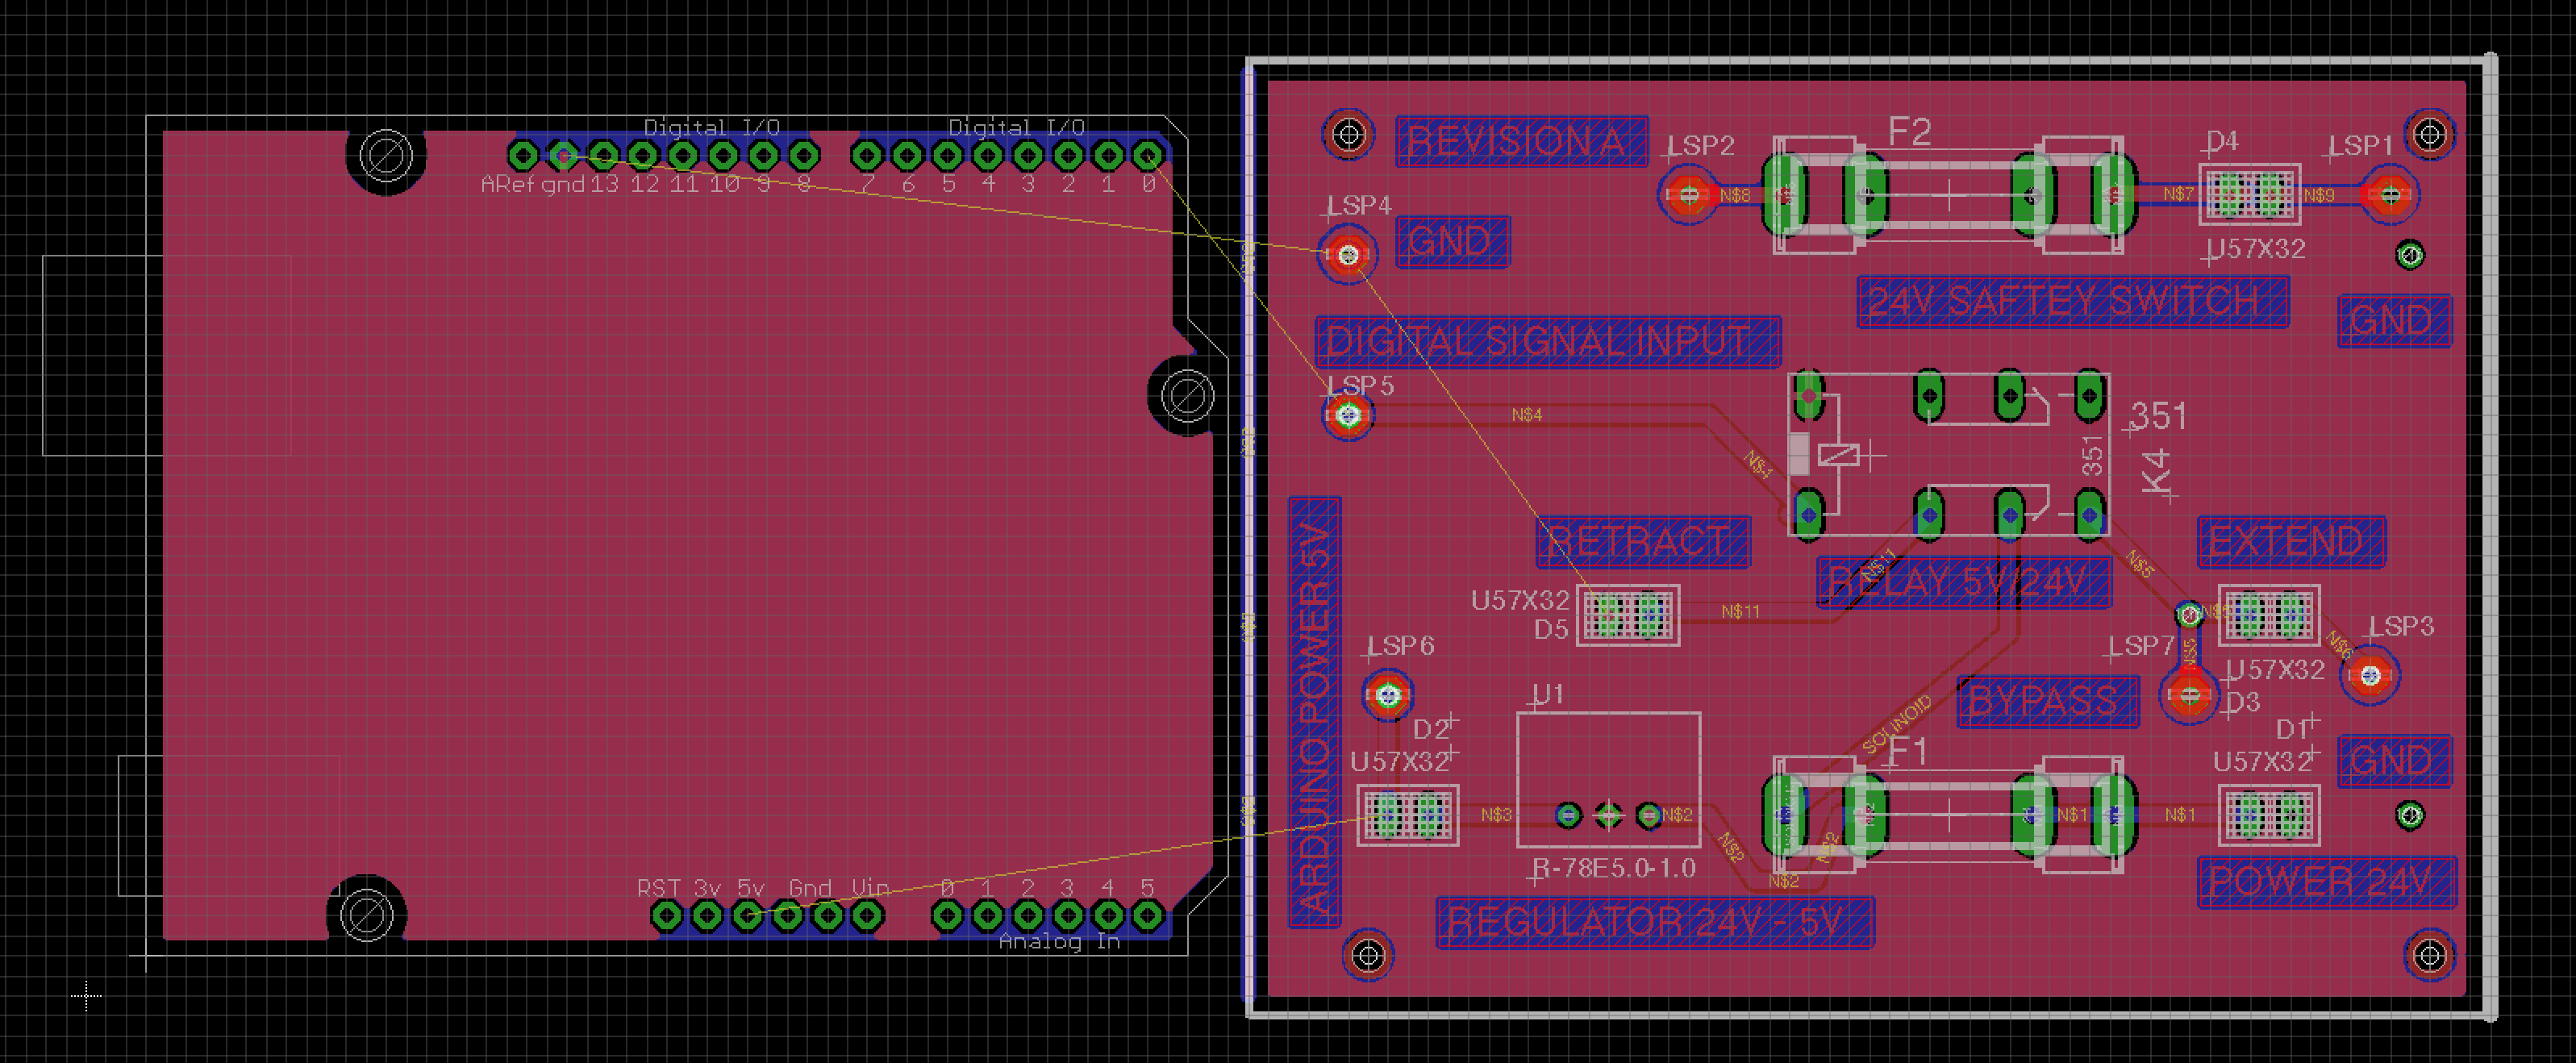
\includegraphics[width=\linewidth]{images/Board}
  \caption{Board design}
  \label{fig:Board design}
\end{figure}

%%%%%%%%%%%%%%%%%%%%%%%%%%%%%%%%%%%%%%%%%%%%%%%%%%%%%%%%%%%%%%%%%%%%%%%%%%%%%%%%

\subsection{Sensor Selection}

In order to measure the distance of the pneumatic actuation arm a form of sensor is acquired. The sensor chosen is the *****, this was selected due to the *********** and the linear properties of the sensors measurement, without issues from depreciation due to limited cycles.

The Actuation is measured with the ******** sensor and sent to the Arduino, which in turn translates the read value from voltage to decimal and is displayed in millimetres on the mounted LCD display located above the Arduino and PCB on the inside of the enclosure. 

%\begin{figure}[H]
%  \includegraphics[width=\linewidth]{images/sensor}
%  \caption{Selected sensor}
%  \label{fig:Selected sensor}
%\end{figure}

%%%%%%%%%%%%%%%%%%%%%%%%%%%%%%%%%%%%%%%%%%%%%%%%%%%%%%%%%%%%%%%%%%%%%%%%%%%%%%%%

\subsection{Programming}

The selected device for use as the controller, and to measure and display the extension is the Arduino Uno. The reasons this was the selected micro-controller board is for no other then being cost effective, as this was taken from past years projects. As there were no specifications on what must be used this was the most appropriate solution.

A summary of the code is shown in the appendix which covers in full the method of deploying the projectiles, the override function, and displaying the displacement of the actuator. Please see the comments embedded in the code for a more step by step detailed explanation for what is being processed.

%%%%%%%%%%%%%%%%%%%%%%%%%%%%%%%%%%%%%%%%%%%%%%%%%%%%%%%%%%%%%%%%%%%%%%%%%%%%%%%%
%%%%%%%%%%%%%%%%%%%%%%%%%%%%%%%%%%%%%%%%%%%%%%%%%%%%%%%%%%%%%%%%%%%%%%%%%%%%%%%%

\section{RESULTS}

The products procedure resulted in a successful build of which a projectile is deployed and given information is passed to the user on a mounted LCD display. All of the objectives sought out to achieve have been completed. The projectiles average range was recorded at ****m when launched from the ground and ****m when launched from 1m above ground level. Below is the finished product captured from two angles.

%\begin{figure}[H]
%  \includegraphics[width=\linewidth]{images/final}
%  \caption{The final product}
%  \label{fig:The final product}
%\end{figure}

%\begin{figure}[H]
%  \includegraphics[width=\linewidth]{images/final2}
%  \caption{The final product side 2}
%  \label{fig:The final product side 2}
%\end{figure}

%%%%%%%%%%%%%%%%%%%%%%%%%%%%%%%%%%%%%%%%%%%%%%%%%%%%%%%%%%%%%%%%%%%%%%%%%%%%%%%%
%%%%%%%%%%%%%%%%%%%%%%%%%%%%%%%%%%%%%%%%%%%%%%%%%%%%%%%%%%%%%%%%%%%%%%%%%%%%%%%%

\section{OUTCOMES}

Successfully achieved and built a mechatronic sub-system using the following

\begin{itemize}
	\item Sensing elements and signal conditioning used within a mechatronic device
	\item Pneumatics and hydraulics
	\item Mechanical and electrical actuators
	\item Integrated mechatronic sub-systems to build a mechatronic device
	\item Configured and use PC and PLC control systems
\end{itemize}

%%%%%%%%%%%%%%%%%%%%%%%%%%%%%%%%%%%%%%%%%%%%%%%%%%%%%%%%%%%%%%%%%%%%%%%%%%%%%%%%

\subsection{Fine Tuning} 

While the process is rudimentary there is much room for fine tuning, this could be in the design of the enclosure, the rate of actuation, the speed, and angle, of which the projectiles are deployed and so on. The range is highly subject to these parameters and is significantly effected from initial launch height so therefore an optimum combination of these can be found depending on the use of the product. After these parameters are established the settings can be tuned and set to random if chosen for a more unexpected distance result if required.

%%%%%%%%%%%%%%%%%%%%%%%%%%%%%%%%%%%%%%%%%%%%%%%%%%%%%%%%%%%%%%%%%%%%%%%%%%%%%%%%

\subsection{Testing}

The main aspects of testing is to show that the devices works and meets the objective criteria. After the projectiles are launch and LCD displayed, details of range can be recorded. A not necessarily obvious, but extremely key part of very necessary testing is the question of practicality; how easy it is to use and understand, is everything simple to understand and labeled correctly, and most importantly, how intuitive is the device. These features are checked over to make sure the device is simple and easy to setup and use, coming all in a single enclosure with enough information to determine functionality with no additional support. 

The device is checked for standalone use, as well as being run via a computer interface terminal. It is easy to update and diagnose, and is simple to connect.

After all the results are finalised, the outputs confirmed with objectives complete, the project is simplified for clarity and ease of use for future development and reference. Making the build stable and concise, and as robust as possible prompts for a good design. Checking over the functions and any redundant features, ensure a good user interface is easily workable and the outputs are all correct and comprehensive.

%%%%%%%%%%%%%%%%%%%%%%%%%%%%%%%%%%%%%%%%%%%%%%%%%%%%%%%%%%%%%%%%%%%%%%%%%%%%%%%%

\subsection{Finalising}

As this is a prototype build a further recommendation coming to a final product design would be to use an ABS mould with rounded edges and an integrated handle with an adjustable deploy angle fitment and 1.5m portable stand. A bluetooth remote would also be handy to start the sequence 0-15m no obstruction range, as an official tennis court is 23.77m long and singles line distance is 10.97m \cite{ball} xtherefore the average range would not exceed 15m once setup; that is if the product were to be used for this purpose.

The main limitation of this device is there is no automatic rotation angle feature, meaning that if someone were to actually purchase this device it might be a key feature in which they seek. Therefore an investigation of how to incorporate this might prove necessary, however due to the scope of this project it is unnecessary to go further into details.

Finally, being as the device is pressure driven, the option of having a replacement induction driven actuator should be considered if used in final product, as it may not be particle to have a compressor or refillable canister always attached.

%%%%%%%%%%%%%%%%%%%%%%%%%%%%%%%%%%%%%%%%%%%%%%%%%%%%%%%%%%%%%%%%%%%%%%%%%%%%%%%%
%%%%%%%%%%%%%%%%%%%%%%%%%%%%%%%%%%%%%%%%%%%%%%%%%%%%%%%%%%%%%%%%%%%%%%%%%%%%%%%%

\section{CONCLUSIONS}

\subsection{Critical Evaluation and Methodology}

%The final transformation of workspaces have been produced from several steps. This demonstration gives the user a guided input and accurate clear output for, easy to use, and self guided results.
%
%As the output for all processed images was found accurate and complete the method has been found effective. The results are clearly given show the center coordinates of both contours, a homogeneous transformation matrix, rotation and translation between characters all displayed to the user as output in terminal, and the final image saved to the output source folder. 

\subsection{Discussion}

%This process preforms and meets all aims and objects set out to achieve and can be considered a success. All required information displayed to the user in an orderly fashion and input methods are acceptable. In achieving this task the demonstration presents a practical form in which by using bounding rectangles, contours and points vectors, a total accurate reformation can be drawn accross a translational span.
%
%The process's used were successfully able to detect and identify all characters, and have been able to take the product of matrices and find significant angles. The transformations have completed all images with speed and accuracy, and is a viable method of detection and transformation.

%%%%%%%%%%%%%%%%%%%%%%%%%%%%%%%%%%%%%%%%%%%%%%%%%%%%%%%%%%%%%%%%%%%%%%%%%%%%%%%%
%%%%%%%%%%%%%%%%%%%%%%%%%%%%%%%%%%%%%%%%%%%%%%%%%%%%%%%%%%%%%%%%%%%%%%%%%%%%%%%%

\nocite{*}
\bibliographystyle{ieeetr}
\bibliography{references}

%%%%%%%%%%%%%%%%%%%%%%%%%%%%%%%%%%%%%%%%%%%%%%%%%%%%%%%%%%%%%%%%%%%%%%%%%%%%%%%%
%%%%%%%%%%%%%%%%%%%%%%%%%%%%%%%%%%%%%%%%%%%%%%%%%%%%%%%%%%%%%%%%%%%%%%%%%%%%%%%%

\clearpage
\onecolumn

\section*{APPENDIX}

\begin{lstlisting}[language = C++]
*******************************************************************************
*******************************************************************************
*******************************************************************************
***********************************************************************
\end{lstlisting}

\end{document}
